\chapter{Two reaction system}

At first, the Monte Carlo algorithm implementation was applied to the most basic -- two reaction test case. We apply it on the model of a plasma composed of three chemical species: argon \ch{Ar},  argon ion \ch{Ar+}, and electron \ch{e-}.

\section{Reactions}

There are only two reactions: argon ionization and recombination. We denote the reaction rates $k_1$ (for argon ionization) and $k_2$ (for recombination).

During the ionization, an electron collides with an electronegative argon atom, causing it to lose an electron:
\ch{e- + Ar ->[ $k_1$ ] e- + e- + Ar+}.

On the other hand, the recombination reaction consists of a ionized argon atom absorbing an electron: 
\ch{e- + Ar+ + Ar ->[ $k_2$ ] Ar + Ar}.

It can be shown that such a system yields an equilibrium, where the electron concentration $\left[ e^{-} \right] = \frac{k_1}{k_2}$ if sufficiently rich in particles. Due to the reaction symmetries, argon ions reach the same concentration; argon atoms then make up the rest of the system.

\section{Numerical solution}

For this test case, the solution is pretty straightforward. First, we construct the corresponding differential equations for the given reactions. Here, $\left[ X\right]_t$ denotes the concentration of element $X$ at time $t$. 

$$ \frac{\dif \left[ \rm e^{-} \right]_t}{\dif t} = k_1\left[ \rm e^{-}\right]_t \left[ \rm Ar\right]_t - k_2 \left[ \rm e^{-}\right]_t \left[ \rm Ar^{+}\right]_t \left[ \rm Ar\right]_t$$

$$\frac{\dif \left[\rm Ar\right]_t}{\dif t} = - k_1\left[ \rm e^{-}\right]_t \left[ \rm Ar\right]_t + k_2 \left[ \rm e^{-}\right]_t \left[ \rm Ar^{+}\right]_t \left[ \rm Ar\right]_t$$

$$\frac{\dif \left[\rm Ar^{+}\right]_t}{\dif t} = k_1\left[ \rm e^{-}\right]_t \left[ \rm Ar\right]_t - k_2 \left[ \rm e^{-}\right]_t \left[ \rm Ar^{+}\right]_t \left[ \rm Ar\right]_t$$

Note, that the right-hand sides of the differential equations evaluate to zero when we set $\left[ \rm e^{-}\right]_t = \left[\rm Ar^{+}\right]_t = \frac{k_1}{k_2}$. This is the concentration equilibrium of the two reaction system. 

If we solve these equations, we obtain the following results. The initial concentrations were chosen to be $\left[e^{-}\right]_0 = \left[Ar^{+}\right]_0 = 1\;\rm cm^{-3}$ and $\left[Ar\right]_0 = 10^{19}\;\rm cm^{-3}$. The reaction rates are constant in this case, taken from the \verb|ZDPlasKin| database; $k_1 = 0.487\cdot10^{-11} \;\rm cm^{3} \rm s^{-1}$, $k_2 = 10^{-25} \;\rm cm^{6} \rm s^{-1}$.

\begin{figure}
    \centering
    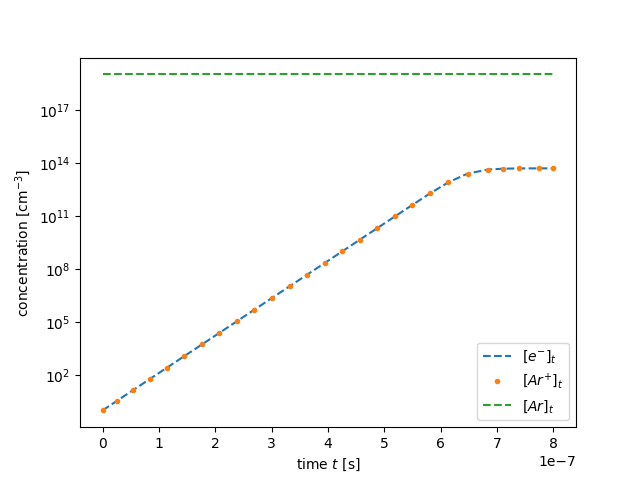
\includegraphics[width=0.9\textwidth]{grafy/2reaction_analytical.png}
    \caption{Two reaction system -- analytical solution}
    \label{fig:my_label}
\end{figure}

\section{Monte Carlo solution}

TODO: add the solution with nice graphs (and delete the fig 3.1 above, merging it with this one).

I wanna mention the results with SIMPLE MC, then maybe comment on different Ns as another subsection?